\section{Results and Analysis}
\label{sec: results}
Table \ref{table: results-acc} shows the accuracy on the testset for each model,
averaged over three runs with different seeds. Several abbreviations
clarification: DCBOW stands for Deep CBOW, DCBOW-PT stands for Deep CBOW with
pretrained embedding, Mini-LSTM means vanilla LSTM trained with minibatch,
T-LSTM stands for Tree-LSTM, ST-LSTM is the tree LSTM trained with per-node
supervision and CS-LSTM refers to Child-Sum LSTM. \\ Table \ref{table: sign}
reflects the significance of these predictions when compared to another model.
The combination of these metrics makes it possible to answer a number of
research questions. \\
% \begin{enumerate}
    % \vspace{-20pt}
    \textit{1. How important is word order for the task of classification of
    sentiment?} To answer this question, one only has to compare the accuracy
    results of BOW-like models and vanilla LSTM. Note that most of the BOW
    models are trained with random embedding initialization, except for
    DCBOW-PT, so it is only fair to compare DCBOW-PT with LSTM. And we can see
    LSTM is about 3 percent over the DCBOW-PT, which is a large gap.
    % \vspace{-7pt}

    \textit{2. Does tree structure improve the accuracy as opposed to
    sequential learning?} We compare the accuracy of both T-LSTM with Mini-LSTM,
    instead of vanilla LSTM, since T-LSTM is also trained in the minibatch way.
    The mean of T-LSTM is over Mini-LSTM by 0.01, but considering the variance
    of both estimations, it is not sufficient to say tree structure brings a
    performance boost. The significance test in Table \ref{table: sign} agrees
    with this view.
    % \vspace{-7pt}

    \textit{3. Performance on supervising sentiment per-node?} 
    In opposite to our hypothesis, imposing supervision per-node on tree LSTM
    results in worse result in terms of mean accuracy on test set. The ST-LSTM
    performs worst among all LSTM models, and according to significance table,
    the difference between ST-LSTM and T-LSTM is not statistically significant.
    It might result from the sparsity per batch and bad hyperparameters.
    However, we do observe less overfit in the training of ST-LSTM, suggesting
    adding per-node supervision might be a good regularizer.
    % \vspace{-7pt}
    
    \textit{4. Will the performance vary much on different sentence length across models?} 
    Figure \ref{fig: results-sent-leng} shows the results for the majority of
    the models on various sentence lengths, averaged over three different
    training instances of each model. The Tree-LSTM almost outperforms all
    models for all sentence-lengths, and achieves highest performance over all
    models in the longer-sentences range, as our initial hypothesis stated.
    However, initial exploration of the data showed a decrease in sample size as
    longer sentences are evaluated, leading to there not being enough evidence
    yet to support the claim that Tree LSTM is significantly better.
    
    \begin{figure}
        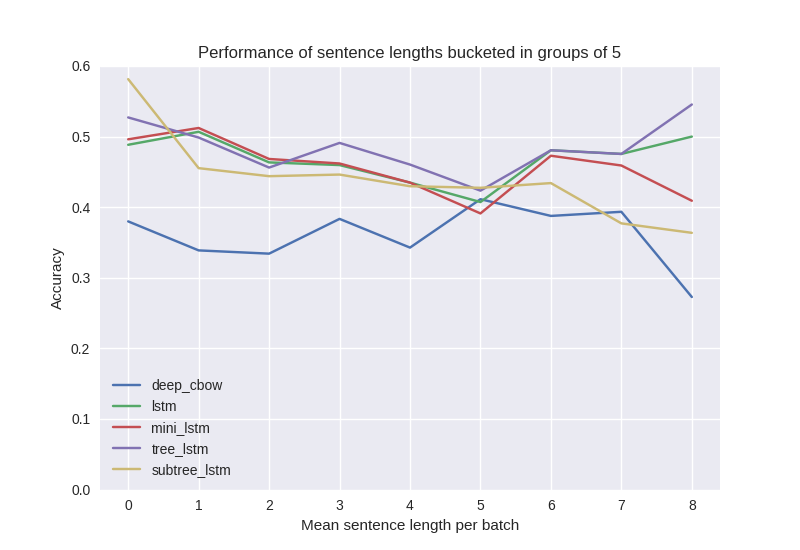
\includegraphics[width=80mm]{assets/Sen_length.png}
        \caption{Mean Performance of sentence lengths }
        \label{fig: results-sent-leng}
    \end{figure}
    % \vspace{-7pt}

    \textit{5. How does N-ary Tree LSTM compare to the Child-Sum Tree LSTM?}
    In opposite to our original hypothesis, the Child-Sum Tree LSTM performs
    competitive with N-ary Tree LSTM in this task. Since each node has only two
    children in our dataset, the order of this two children might not be as
    useful as we previously thought. For example, when the left and right child
    are "this movie" and "is nauseous" respectly, whichever order they are
    composed will not change the final inference result too much. The reasons
    can also lie in the choice of hyperparameter, especially in learning rate. 
% \end{enumerate}
